\documentclass[aspectratio=169]{beamer}

% Shared Beamer settings for Applied Machine Learning lectures (UPES).
% Keep this file free of \documentclass to allow reuse via \input.

% Allow lecture sources to use shared theme/assets without copying them into each lecture folder.
% NOTE: These paths are relative to `Unit-xx/Lecture-yy/latex/` (and `Lab/Experiment-xx/latex/`).
\makeatletter
\def\input@path{{../../../_shared/}{../../../_shared/UPES-Beamer-Theme/}}
\makeatother

\usetheme{UPES}
\setbeamertemplate{navigation symbols}{}

\usepackage{amsmath}
\usepackage{amssymb}
\usepackage{booktabs}
\usepackage{graphicx}
\usepackage{hyperref}
\usepackage{xcolor}
\usepackage{listings}

% Code listings (Python-oriented for this subject).
\lstset{
  language=Python,
  basicstyle=\ttfamily\small,
  keywordstyle=\color{blue},
  commentstyle=\color{gray},
  stringstyle=\color{teal},
  showstringspaces=false,
  columns=fullflexible,
  breaklines=true
}

\usepackage{tikz}
\usetikzlibrary{arrows.meta,positioning,shapes.geometric,calc,fit,backgrounds}

% Per-slide source line (references shown on the slide itself).
\newcommand{\slidesources}[1]{%
  \vfill
  {\tiny\color{gray}\raggedright\sloppy\parbox{\linewidth}{Sources: #1}\par}%
}

% Unit-wise source strings for this subject (used by slides/notes).
% Path is relative to the lecture `latex/` folder (the compilation CWD).
% Source strings for Applied Machine Learning (CSAI2017P) — used by slides + notes.
% Prescribed texts and reference books are taken from the course syllabus.
% Support texts are the author-hosted open-access editions:
%   statlearning.com            (ISL with Python)
%   probml.github.io/pml-book   (Murphy, Probabilistic Machine Learning)
%   d2l.ai                      (Dive into Deep Learning)
%   mml-book.github.io          (Mathematics for Machine Learning)

\newcommand{\AMLRepoURL}{https://github.com/tali7c/Applied-Machine-Learning}

% --- prescribed -------------------------------------------------------------
\newcommand{\AMLPrescribed}{%
M\"uller and Guido, \textit{Introduction to Machine Learning with Python}, O'Reilly, 2016.;%
Bishop, \textit{Pattern Recognition and Machine Learning}, Springer, 2006.;%
Murphy, \textit{Machine Learning: A Probabilistic Perspective}, MIT Press, 2012.;%
Han, Kamber and Pei, \textit{Data Mining: Concepts and Techniques} (3e), Morgan Kaufmann, 2012.%
}

% --- unit-wise ---------------------------------------------------------------
\newcommand{\AMLUnitISources}{%
M\"uller and Guido, \textit{Introduction to Machine Learning with Python}, Ch. 1.;%
Bishop, \textit{Pattern Recognition and Machine Learning}, Ch. 1.;%
Murphy, \textit{Probabilistic Machine Learning: An Introduction}, MIT Press, 2022, Ch. 1.;%
Mitchell, \textit{Machine Learning}, McGraw Hill, 1997, Ch. 1.;%
Scikit-learn documentation, accessed 2026-08-04.%
}

\newcommand{\AMLUnitIISources}{%
Bishop, \textit{Pattern Recognition and Machine Learning}, \S1.5, \S4.3, \S7.1.;%
Zhang, Lipton, Li and Smola, \textit{Dive into Deep Learning}, \S3.4.;%
Shalev-Shwartz and Ben-David, \textit{Understanding Machine Learning}, Ch. 15.;%
Murphy, \textit{Probabilistic Machine Learning: An Introduction}, Ch. 5.%
}

\newcommand{\AMLUnitIIISources}{%
Zhang, Lipton, Li and Smola, \textit{Dive into Deep Learning}, Ch. 12 (Optimization Algorithms).;%
Deisenroth, Faisal and Ong, \textit{Mathematics for Machine Learning}, Ch. 7.;%
Kingma and Ba, ``Adam: A Method for Stochastic Optimization,'' ICLR 2015.;%
Ruder, ``An overview of gradient descent optimization algorithms,'' arXiv:1609.04747, 2016.%
}

\newcommand{\AMLUnitIVSources}{%
Han, Kamber and Pei, \textit{Data Mining: Concepts and Techniques} (3e), Ch. 3.;%
M\"uller and Guido, \textit{Introduction to Machine Learning with Python}, Ch. 3--4.;%
James, Witten, Hastie, Tibshirani and Taylor, \textit{An Introduction to Statistical Learning with Python}, Ch. 5--6, 12.;%
Scikit-learn documentation (preprocessing, model selection), accessed 2026-08-04.%
}

\newcommand{\AMLUnitVSources}{%
James et al., \textit{An Introduction to Statistical Learning with Python}, Ch. 3--6.;%
Bishop, \textit{Pattern Recognition and Machine Learning}, Ch. 3.;%
Deisenroth, Faisal and Ong, \textit{Mathematics for Machine Learning}, Ch. 9.;%
M\"uller and Guido, \textit{Introduction to Machine Learning with Python}, \S2.3.%
}

\newcommand{\AMLUnitVISources}{%
Han, Kamber and Pei, \textit{Data Mining: Concepts and Techniques} (3e), Ch. 8--9.;%
James et al., \textit{An Introduction to Statistical Learning with Python}, Ch. 8--9.;%
Bishop, \textit{Pattern Recognition and Machine Learning}, Ch. 4--5, 7, 14.;%
Zhang et al., \textit{Dive into Deep Learning}, Ch. 5.%
}

\newcommand{\AMLUnitVIISources}{%
Han, Kamber and Pei, \textit{Data Mining: Concepts and Techniques} (3e), Ch. 10.;%
James et al., \textit{An Introduction to Statistical Learning with Python}, Ch. 12.;%
M\"uller and Guido, \textit{Introduction to Machine Learning with Python}, \S3.5.;%
Ester, Kriegel, Sander and Xu, ``A density-based algorithm for discovering clusters (DBSCAN),'' KDD 1996.%
}

\newcommand{\AMLLabSources}{%
M\"uller and Guido, \textit{Introduction to Machine Learning with Python}, companion notebooks.;%
McKinney, \textit{Python for Data Analysis} (3e), O'Reilly, 2022.;%
Scikit-learn user guide, accessed 2026-08-04.;%
Matplotlib and Seaborn documentation, accessed 2026-08-04.%
}



\graphicspath{{../figures/}{../images/}{../../../_shared/}{../../../_shared/UPES-Beamer-Theme/}}

\title[Applied Machine Learning]{Applied Machine Learning}
\subtitle{Unit 07 -- Lecture 24: Course Revision and Consolidation}
\author{Tofik Ali}
\institute{School of Computer Science, UPES Dehradun}
\date{Autumn 2026}

% ---- a compact "output" block so code and its result sit together ----------
\lstdefinestyle{outblk}{
  basicstyle=\ttfamily\scriptsize\color{black!75},
  backgroundcolor=\color{black!5}, frame=leftline, framerule=2pt,
  rulecolor=\color{black!30}, breaklines=true, columns=fullflexible,
  keepspaces=true,   % several outputs below are aligned tables
  language={},       % printed output is not Python: do not syntax-highlight it
  xleftmargin=4pt, aboveskip=1pt, belowskip=1pt, literate={-}{{-}}1}
\lstnewenvironment{outblk}{\lstset{style=outblk}}{}

\begin{document}

\UPESCoverFrame
\setcounter{framenumber}{0}

\begin{frame}
  \titlepage
  \begin{center}
    \footnotesize Seven units, one argument.\\[0.25em]
    \footnotesize Topic focus: \textbf{which method, and how would you know
      you were wrong}\\[0.25em]
    \footnotesize Repository: \texttt{\AMLRepoURL}
  \end{center}
  \slidesources{\AMLPrescribed}
\end{frame}

\begin{frame}{Quick Links}
  \centering
  \hyperlink{sec:spine}{\beamerbutton{The spine}}\hspace{0.4em}
  \hyperlink{sec:zoo}{\beamerbutton{One dataset, every model}}\hspace{0.4em}
  \hyperlink{sec:choose}{\beamerbutton{Choosing}}\hspace{0.4em}
  \hyperlink{sec:mistakes}{\beamerbutton{Five mistakes}}\\[0.6em]
  \hyperlink{sec:e2e}{\beamerbutton{End to end}}\hspace{0.4em}
  \hyperlink{sec:hand}{\beamerbutton{The arithmetic that recurs}}\hspace{0.4em}
  \hyperlink{sec:map}{\beamerbutton{Revision map}}\\[0.6em]
  \hyperlink{sec:assess}{\beamerbutton{What is left to be assessed}}\hspace{0.4em}
  \hyperlink{sec:summary}{\beamerbutton{Summary}}
\end{frame}

\begin{frame}{Agenda}
  \tableofcontents
\end{frame}

\begin{frame}[shrink=8]{How this lecture works}
  \begin{columns}[T]
    \begin{column}{0.48\textwidth}
      \begin{block}{This is not a list of topics}
        You already have twenty-three sets of notes that list topics. The job
        today is to turn them into \textbf{one argument}, so that when you
        are handed a problem you have never seen you can say which method to
        try, why, and what would tell you it was the wrong choice.
      \end{block}
    \end{column}
    \begin{column}{0.48\textwidth}
      \begin{alertblock}{Commit before you look}
        Five slides ask you to choose a method, or to find the error in a
        block of code, \emph{before} the answer appears. These are
        diagnostic. Getting one wrong now is cheap; getting it wrong in an
        examination is not.
      \end{alertblock}
    \end{column}
  \end{columns}
  \vspace{0.3em}
  \begin{center}
    \small Everything quoted today was \textbf{re-measured for this lecture}
    under one protocol --- one dataset, one pipeline, twenty folds --- rather
    than copied from the earlier packages.
  \end{center}
\end{frame}

\begin{frame}{One seed for the whole revision, and two sweeps}
  \begin{columns}[T]
    \begin{column}{0.48\textwidth}
      \begin{block}{The randomness}
        \small One seed: \texttt{random\_state=24} and
        \texttt{np.random.default\_rng(24)}. Every model, every split, every
        shuffle, every synthetic set. The outer loop of a nested CV uses
        \texttt{25} so that it is not the inner loop.
      \end{block}
    \end{column}
    \begin{column}{0.48\textwidth}
      \begin{block}{Two sweeps}
        \small Mistakes 1 and 2 are measured on \textbf{twenty fresh noise
        problems} each, from two different streams. One trial of a noise
        experiment proves nothing.
      \end{block}
    \end{column}
  \end{columns}
  \vspace{0.5em}
  \begin{alertblock}{The one thing a seed cannot fix}
    \centering\small
    Every number in this deck reproduces exactly \emph{except the
    milliseconds}. Quote what is countable --- $3201$ weights against $31$
    coefficients, $100$ trees, $106$ support vectors --- never the clock.
  \end{alertblock}
\end{frame}

% =====================================================================
\section[The spine]{Seven units, one argument}
\label{sec:spine}

\begin{frame}[shrink=5]{The four questions the whole course answers}
  \begin{columns}[T]
    \begin{column}{0.49\textwidth}
      \begin{enumerate}
        \item \textbf{What quantity are we minimising?} \hfill Unit II
        \item \textbf{How is the minimisation carried out?} \hfill Unit III
        \item \textbf{Over what class of functions?} \hfill Units V, VI
        \item \textbf{How would I know it worked?} \hfill Units IV and VI
      \end{enumerate}
      \vspace{0.4em}
      And before all four: \textbf{what do you feed it?} --- Unit IV again,
      because the columns you supply decide what the optimiser can possibly
      find.
    \end{column}
    \begin{column}{0.49\textwidth}
      \begin{exampleblock}{Unit VII is the same picture with a hole in it}
        Delete the target column and questions 1 and 4 both lose their
        meaning. There is no loss to minimise and nothing to score against.
        What replaces the loss is a \emph{distance}, and what replaces the
        score is your own stated assumption.
      \end{exampleblock}
      \begin{alertblock}{The sentence to carry out of the room}
        Least squares, logistic regression, trees, forests, boosting,
        networks and SVMs are \textbf{not seven inventions}. They are one
        recipe with the hypothesis class and the loss swapped out.
      \end{alertblock}
    \end{column}
  \end{columns}
\end{frame}

\begin{frame}{The whole course on one page}
  \begin{center}
    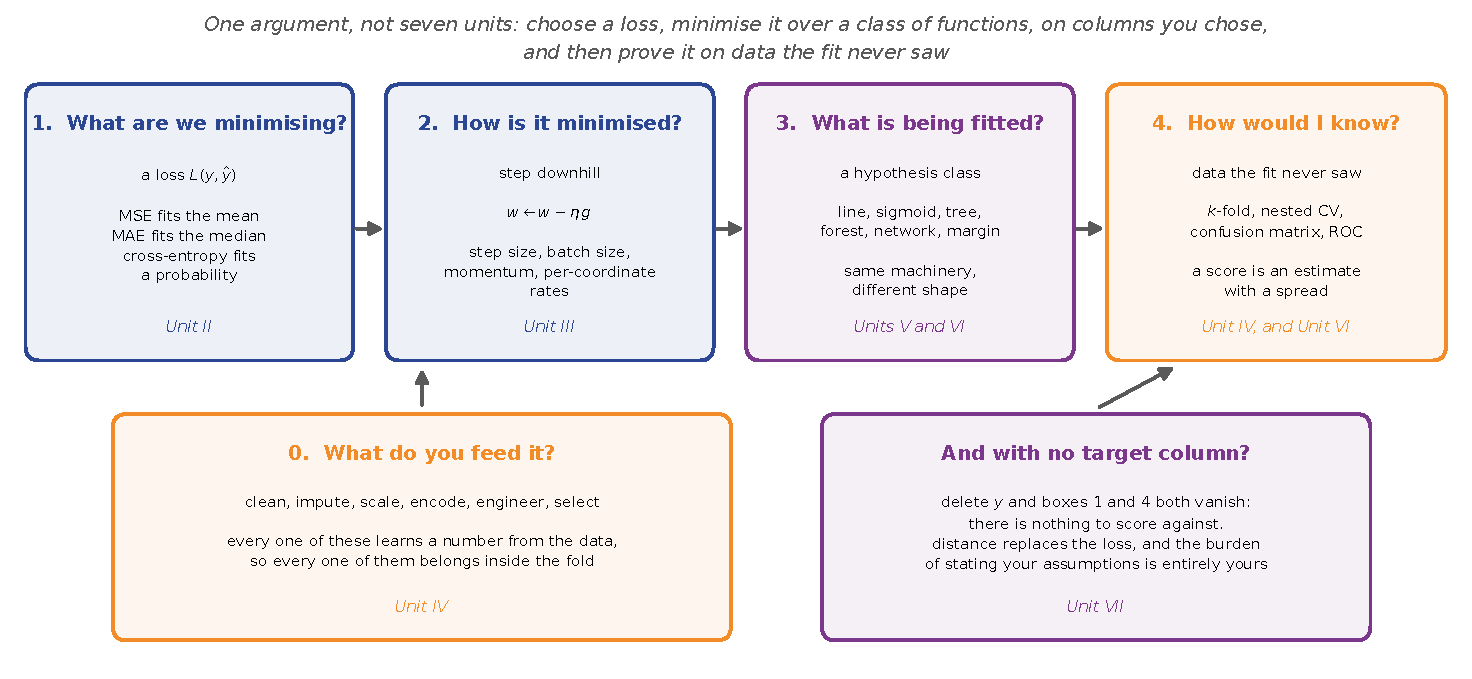
\includegraphics[width=0.98\textwidth,height=0.80\textheight,keepaspectratio]{spine.pdf}
  \end{center}
\end{frame}

\begin{frame}[shrink=10]{Same recipe, seven fillings}
  \centering
  \begin{tabular}{@{}llll@{}}
    \toprule
    \textbf{Method} & \textbf{Hypothesis class} & \textbf{Loss} &
      \textbf{Minimised by} \\
    \midrule
    Least squares      & linear in $x$      & squared error    & closed form \\
    Ridge / lasso      & linear in $x$      & squared $+$ penalty & closed form / coordinate descent \\
    Logistic           & linear in log-odds & cross-entropy    & gradient descent, IRLS \\
    Decision tree      & axis-aligned boxes & impurity drop    & greedy search \\
    Random forest      & average of trees   & impurity drop    & greedy $+$ bootstrap \\
    Boosting           & sum of trees       & any differentiable & stagewise gradient \\
    Neural network     & composed layers    & any differentiable & backpropagation $+$ SGD \\
    SVM                & linear in a feature map & hinge $+$ $\lVert w\rVert^2$ & convex QP \\
    $k$-NN             & the training table & --- (no fit)     & --- \\
    \bottomrule
  \end{tabular}
  \vspace{0.5em}
  \begin{center}
    \small Read the table \emph{down the columns}, not across the rows. Every
    row is the same three decisions.
  \end{center}
\end{frame}

\begin{frame}[shrink=8]{What each unit actually established}
  \begin{columns}[T]
    \begin{column}{0.49\textwidth}
      \begin{block}{Unit II --- the loss is a choice}
        Six readings, one corrupted: the MSE-minimising constant moves from
        $12.33$ to $25.67$, past every clean observation. The MAE-minimising
        constant does not move at all.
      \end{block}
      \begin{block}{Unit III --- descent is three questions}
        How big a step, from how much data, with how much memory. At
        $\eta = 1.00$ the iterates cycle $0 \to 6 \to 0$; at $\eta = 1.05$
        they reach $-17.18$ in twenty steps.
      \end{block}
    \end{column}
    \begin{column}{0.49\textwidth}
      \begin{block}{Unit IV --- the input decides the ceiling}
        Select features with the labels before cross-validating and 500
        pure-noise columns score $0.8475$; inside a \texttt{Pipeline},
        $0.5342$.
      \end{block}
      \begin{block}{Units V and VI --- classes and losses}
        Same optimiser, different shapes. Unit VII removes the target and
        makes the distance the whole decision: $k$-means on raw
        \texttt{wine} scores ARI $0.3711$, standardised $0.8975$.
      \end{block}
    \end{column}
  \end{columns}
\end{frame}

% =====================================================================
\section[One dataset]{One dataset, every model}
\label{sec:zoo}

\begin{frame}[fragile]{The protocol, written once and used for everything}
\begin{lstlisting}
X, y = load_breast_cancer(return_X_y=True)          # 569 x 30, 357 benign
cv = RepeatedStratifiedKFold(n_splits=5, n_repeats=4, random_state=24)

for name, est in seven_models.items():
    pipe = Pipeline([("sc", StandardScaler()), ("m", est)])
    # fit on 4/5, score on 1/5, twenty times; the scaler is refitted each time
\end{lstlisting}
  \begin{center}
    \small Twenty folds, not five, so that the fold-to-fold spread is
    measurable rather than guessed. The scaler is \emph{inside} the pipeline,
    which is the whole point of Unit IV.
  \end{center}
  \begin{alertblock}{The question this experiment exists to settle}
    When two models differ by a few thousandths, is that a difference?
  \end{alertblock}
\end{frame}

\begin{frame}[shrink=6]{Predict first \#1}
  \begin{block}{Commit to an answer}
    Seven models --- logistic regression, $k$-NN, a single tree, a random
    forest, gradient boosting, an MLP and an RBF SVM --- on 569 patients and
    30 columns, in one honest cross-validated pipeline.
    \begin{enumerate}
      \item Which wins on \textbf{accuracy}?
      \item Which wins on \textbf{AUC}?
      \item How large is the gap between the top two, and how large is the
        fold-to-fold standard deviation?
    \end{enumerate}
  \end{block}
  \onslide<2->{
  \begin{exampleblock}{Reveal}
    Accuracy: \textbf{logistic regression, 0.9767}. AUC: \textbf{the RBF SVM,
    0.9956}. The AUC gap to second place is \textbf{0.0013}; the fold-to-fold
    standard deviation is \textbf{0.0046}. The gap is about a quarter of the
    noise. \textbf{Four of the seven} models sit within one fold-standard-%
    deviation of the best accuracy.
  \end{exampleblock}}
\end{frame}

\begin{frame}[fragile]{The measured table}
\begin{outblk}
model                    acc      sd     AUC      sd   fit ms  pred ms
LogisticRegression    0.9767  0.0096  0.9943  0.0059      2.3     0.24
KNN (k=11)            0.9675  0.0179  0.9898  0.0077      0.6     1.39
DecisionTree          0.9324  0.0191  0.9290  0.0198      6.1     0.35
RandomForest          0.9626  0.0163  0.9899  0.0073    341.3     7.08
GradientBoosting      0.9605  0.0212  0.9908  0.0085    366.9     0.62
MLP (100,)            0.9767  0.0122  0.9939  0.0067    225.9     0.44
SVM (RBF)             0.9745  0.0099  0.9956  0.0046      2.5     0.71
\end{outblk}
  \begin{center}
    \small Six of the seven are separated by less than $0.017$ of accuracy.
    The seventh --- the single unpruned tree --- is the only one that is
    clearly worse, and it is also the only one with no averaging or
    regularization anywhere in it. \alert{The two millisecond columns are a
    measurement on one machine; the accuracies are not.}
  \end{center}
\end{frame}

\begin{frame}{Drawn: the seven, with the fold cloud behind them}
  \begin{center}
    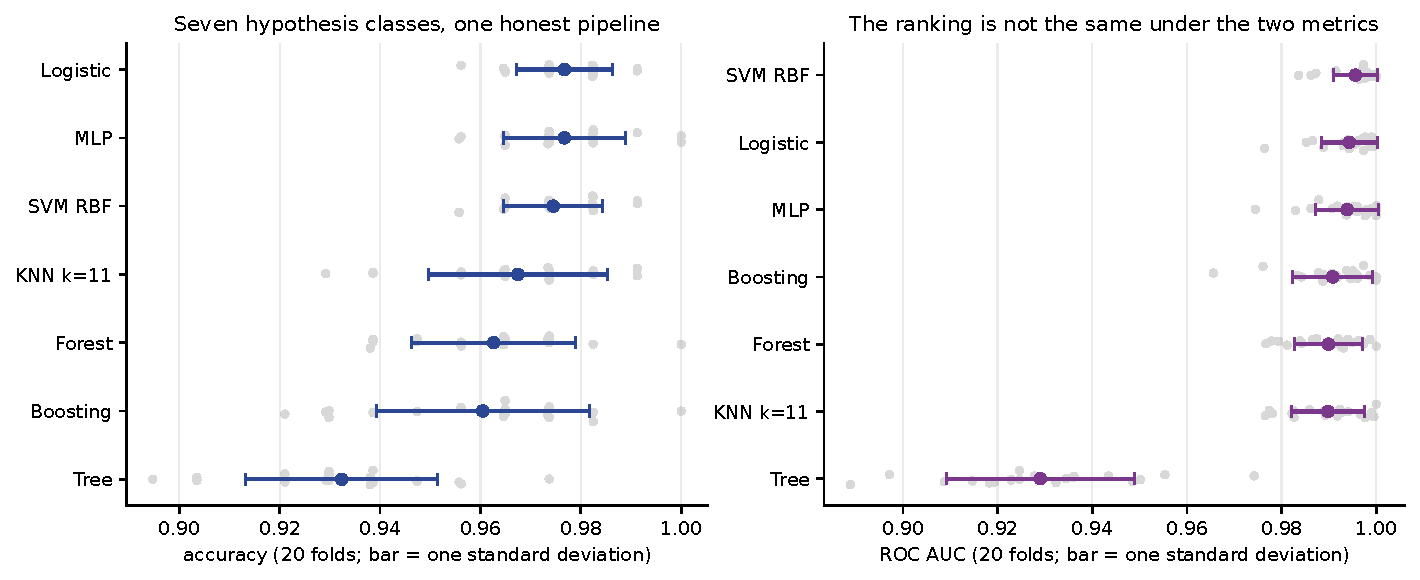
\includegraphics[width=0.95\textwidth,height=0.66\textheight,keepaspectratio]{allmodels.pdf}
  \end{center}
  \vspace{-0.4em}
  \begin{center}
    \small The grey dots are the individual folds. The bars overlap almost
    completely.
  \end{center}
\end{frame}

\begin{frame}[shrink=6]{Predict first \#2 --- is 0.0013 a difference?}
  \begin{block}{Commit}
    The SVM's mean AUC beats logistic regression's by $0.0013$, over twenty
    paired folds. A paired $t$-test gives $p = 0.0232$.
    \emph{Would you report the SVM as the better model?}
  \end{block}
  \onslide<2->{
  \begin{exampleblock}{Reveal}
    The test is significant and the difference is \textbf{immaterial}. The
    nominal winner \textbf{lost 6 of the 20 folds}. On accuracy the same two
    models differ by $+0.0022$ in the \emph{other} direction, with a paired
    $t$-test $p = 0.3965$: logistic wins 7 folds, loses 4 and \textbf{ties 9}.
  \end{exampleblock}}
  \onslide<3->{
  \begin{alertblock}{The rule}
    \textbf{A difference smaller than the fold-to-fold spread is not a
    difference.} Report the spread whenever you report the score, and prefer
    the cheaper or the more interpretable model when the intervals overlap.
  \end{alertblock}}
\end{frame}

\begin{frame}{Drawn: the gap against the spread}
  \begin{center}
    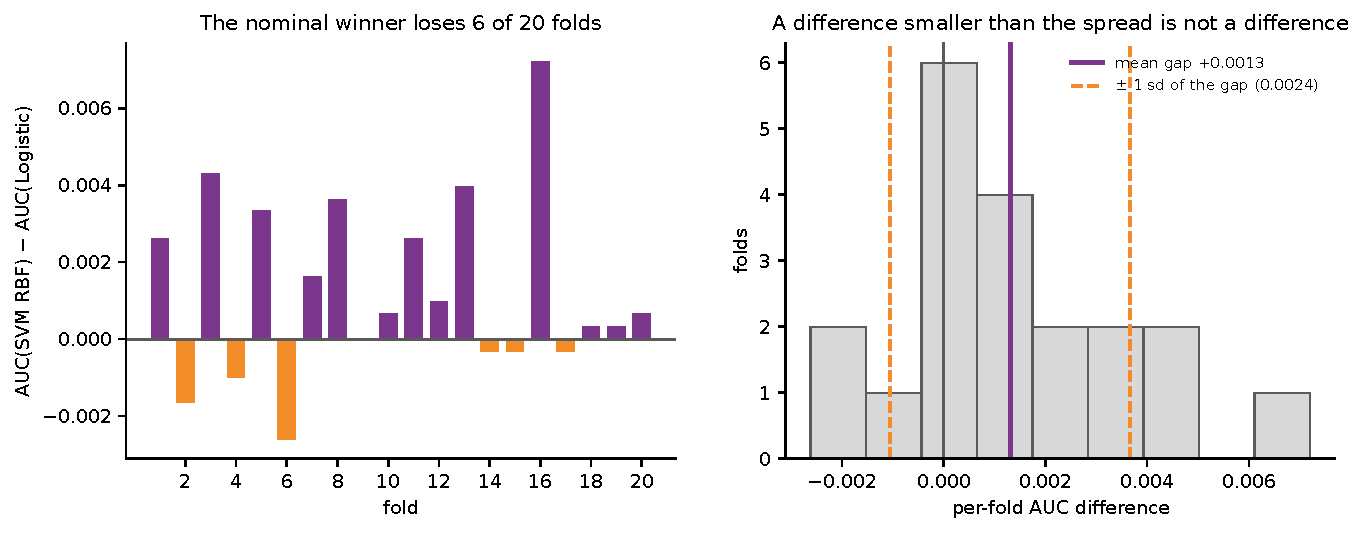
\includegraphics[width=0.93\textwidth,height=0.78\textheight,keepaspectratio]{spread.pdf}
  \end{center}
\end{frame}

\begin{frame}[shrink=5]{And what the seven cost}
  \begin{center}
    
\includegraphics[width=0.78\textwidth,height=0.58\textheight,keepaspectratio]{cost.pdf}
  \end{center}
  \vspace{-0.5em}
  \begin{center}
    \small \textbf{100 trees and 1406 nodes} of gradient boosting buy nothing
    measurable over \textbf{31 coefficients} of logistic regression. $k$-NN is
    the mirror image: nothing fitted, dearest to predict. (Counts, not
    seconds --- the seconds are machine-dependent.)
  \end{center}
\end{frame}

\begin{frame}[fragile,shrink=5]{The ranking depends on the metric}
\begin{outblk}
rank  by accuracy           by AUC
1     LogisticRegression    SVM (RBF)
2     MLP (100,)            LogisticRegression
3     SVM (RBF)             MLP (100,)
4     KNN (k=11)            GradientBoosting
5     RandomForest          RandomForest
6     GradientBoosting      KNN (k=11)
7     DecisionTree          DecisionTree
models whose rank changes with the metric : 5 of 7
\end{outblk}
  \begin{center}
    \small \textbf{Five of seven models change rank} when you change the
    metric. There is no metric-free notion of ``the best model'' --- so name
    the metric before you name the winner, and choose the metric from the
    problem, not from the leaderboard.
  \end{center}
\end{frame}

% =====================================================================
\section[Choosing]{Which method, and why}
\label{sec:choose}

\begin{frame}[shrink=4]{Choosing is not folklore --- every row here is a number}
  \begin{center}
    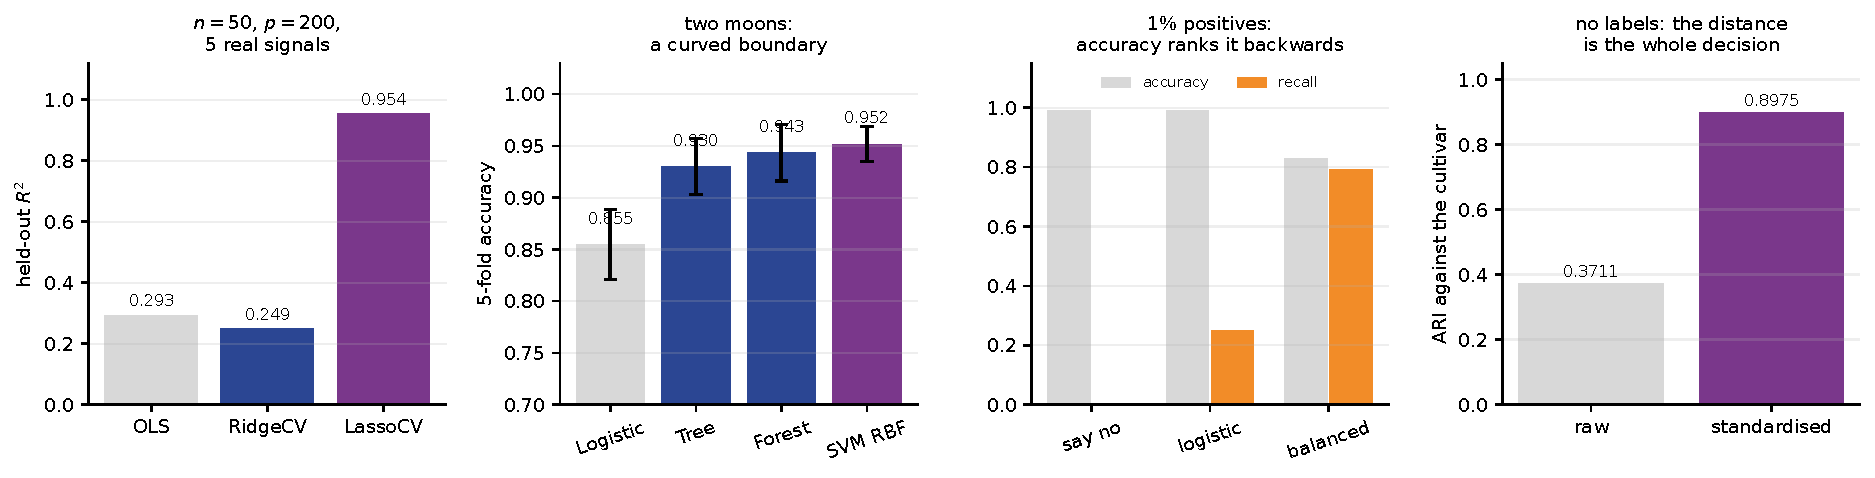
\includegraphics[width=0.99\textwidth,height=0.62\textheight,keepaspectratio]{regimes.pdf}
  \end{center}
  \vspace{-0.3em}
  \begin{center}
    \small Four regimes in which the seven models are \emph{not}
    interchangeable. In each one the choice is worth far more than any
    hyper-parameter sweep.
  \end{center}
\end{frame}

\begin{frame}[shrink=12]{The choosing table}
  \centering
  \begin{tabular}{@{}p{3.0cm}p{3.4cm}p{7.4cm}@{}}
    \toprule
    \textbf{Situation} & \textbf{Try first} & \textbf{Because, measured} \\
    \midrule
    Few rows, many
    columns, sparse truth &
    lasso, then elastic net &
    $n=50$, $p=200$, five real signals: OLS $R^2 = +0.2926$, ridge
    $+0.2492$, lasso $\mathbf{+0.9543}$ and it recovered
    \textbf{5 of the 5} real columns \\[0.3em]
    Interpretability
    required &
    penalised logistic or a shallow tree &
    on \texttt{breast\_cancer}, 30 readable coefficients score AUC $0.9947$
    against gradient boosting's $0.9919$: the readable model cost
    \textbf{nothing} \\[0.3em]
    Non-convex boundary &
    RBF SVM, $k$-NN, or a forest &
    two moons: logistic $0.8550$, tree $0.9300$, forest $0.9433$, SVM
    $\mathbf{0.9517}$ \\[0.3em]
    Heavy imbalance &
    any model, but change the \emph{metric} and the \emph{threshold} &
    at 1\% positives, always-say-no scores accuracy $0.9900$; the model that
    finds 19 of 24 positives scores $0.8275$ \\[0.3em]
    No labels at all &
    clustering, and spend the effort on the distance &
    $k$-means on \texttt{wine}: raw ARI $0.3711$, standardised
    $\mathbf{0.8975}$ --- one column carried $99.77\%$ of the raw variance \\[0.3em]
    Very many rows &
    linear models, or a forest if you can wait &
    40,000 rows: logistic fits in $\mathbf{0.04}$ s, the forest in $10.86$ s,
    the SVM in $5.32$ s and predicts in $2.54$ s \\
    \bottomrule
  \end{tabular}
\end{frame}

\begin{frame}[shrink=6]{Predict first \#3 --- four described problems}
  \begin{block}{Commit to one method for each, and to one reason}
    \begin{enumerate}
      \item 80 patients, 12{,}000 gene-expression columns, and you must tell
        the clinician \emph{which} genes.
      \item 2 million rows, 15 columns, a prediction must return in
        under a millisecond.
      \item 3{,}000 transactions, 30 of them fraudulent, and a missed fraud
        costs a hundred times a false alarm.
      \item 50{,}000 customer records with no label of any kind, and the
        marketing team wants ``segments''.
    \end{enumerate}
  \end{block}
  \onslide<2->{
  \begin{exampleblock}{Reveal}
    \textbf{1} lasso or elastic net --- it is the only family that returns a
    \emph{list}; ridge never returns a zero, its smallest coefficient on a
    swept path was $1.455 \times 10^{-3}$.
    \textbf{2} logistic regression --- not $k$-NN, whose predict cost grows
    with $n$ ($1.11$ ms $\to$ $25.56$ ms for $40\times$ the rows).
    \textbf{3} any model, plus average precision, plus a threshold from the
    10:1 cost --- \emph{not} accuracy.
    \textbf{4} $k$-means or DBSCAN, but first standardise and be able to
    defend the distance; and say out loud that there is no answer key.
  \end{exampleblock}}
\end{frame}

\begin{frame}[shrink=6]{Two answers that are always wrong}
  \begin{alertblock}{``I tried all of them and picked the best score''}
    That is a hyper-parameter search with the test set as the objective. On
    100 rows of pure noise a 22-way model search reports
    $\mathbf{0.5750}$ against a nested $0.5235$, when the truth is $0.5000$
    --- and it overstates on \textbf{17 of 20} trials.
  \end{alertblock}
  \begin{alertblock}{``Deep learning, because it is the most powerful''}
    On these 569 patients the MLP scores $0.9767$ and logistic regression
    scores $0.9767$ --- identical to four decimals --- and the MLP costs
    $\mathbf{103\times}$ as many parameters ($3201$ against $31$). Capacity you do not need is capacity
    you have to regularise, tune and defend.
  \end{alertblock}
  \begin{center}
    \small The defensible answer names a property of the \emph{problem}
    ---~$p \gg n$, curved boundary, prevalence, cost asymmetry, the need to
    explain~--- and then names the family that property implies.
  \end{center}
\end{frame}

% =====================================================================
\section[Five mistakes]{The five mistakes that cost the most}
\label{sec:mistakes}

\begin{frame}{Four of the five, measured}
  \begin{center}
    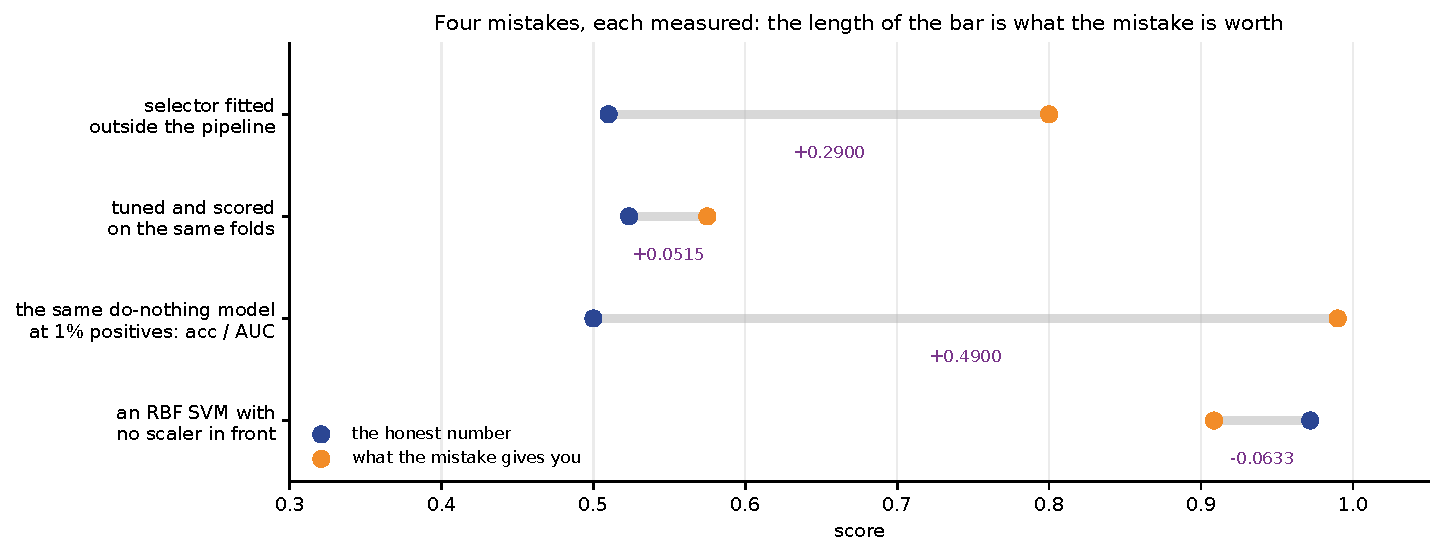
\includegraphics[width=0.88\textwidth,height=0.68\textheight,keepaspectratio]{mistakes.pdf}
  \end{center}
  \vspace{-0.4em}
  \begin{center}
    \small The fifth is not a score at all: it is reading a coefficient as a
    cause.
  \end{center}
\end{frame}

\begin{frame}[fragile,shrink=4]{Mistake 1 --- a transformer fitted outside the pipeline}
\begin{lstlisting}
X = rng.normal(size=(100, 500))      # 500 columns of pure noise
y = rng.integers(0, 2, size=100)     # coin-flip labels: truth is 0.5

sel  = SelectKBest(f_classif, k=10).fit(X, y)   # <-- sees every row
wrong = cross_val_score(LogisticRegression(), sel.transform(X), y, cv=5)

right = cross_val_score(Pipeline([("k", SelectKBest(f_classif, k=10)),
                                  ("m", LogisticRegression())]), X, y, cv=5)
\end{lstlisting}
\begin{outblk}
selection outside the pipeline   0.8000
selection inside the pipeline    0.5100
overstatement                    +0.2900
over 20 fresh noise problems: leaky 0.7535, honest 0.5000
the leaky protocol scored higher on 20 of 20
\end{outblk}
\end{frame}

\begin{frame}[shrink=6]{Why that happens, in one sentence}
  \begin{block}{The mechanism}
    \texttt{SelectKBest} looked at the labels of \emph{every} row, including
    the rows that later became the validation fold. Ten of five hundred
    coin-flip columns will always look predictive by chance --- and once they
    have been chosen using the answers, the validation fold is no longer
    unseen.
  \end{block}
  \begin{alertblock}{The rule that covers all of Unit IV in one line}
    \textbf{Anything that learns a number from the data --- a mean, a median,
    a category list, a rotation, a feature subset, a resampled row, a
    hyper-parameter --- is part of the model and belongs inside the fold.}
  \end{alertblock}
  \begin{center}
    \small The costs measured across the course: leaking a scaler $+0.0034$;
    leaking an imputer, nothing measurable; leaking a row-dropping decision
    $+0.1702$ of $R^2$; resampling before the split, $F_1 = 0.8942$ against
    an honest $0.1133$.
  \end{center}
\end{frame}

\begin{frame}[fragile,shrink=4]{Mistake 2 --- tuning and evaluating on the same folds}
\begin{lstlisting}
gs = GridSearchCV(pipe, grid_of_22_models, cv=inner).fit(X, y)
print(gs.best_score_)                      # <-- this is a MAXIMUM

nested = cross_val_score(GridSearchCV(pipe, grid_of_22_models, cv=inner),
                         X, y, cv=outer)   # <-- this is an ESTIMATE
\end{lstlisting}
\begin{outblk}
breast_cancer   best_score_ 0.9824   nested 0.9824 +/- 0.0125
                optimism    -0.0000
100x30 pure noise, coin-flip labels, 20 trials; truth 0.5000
  best_score_ 0.5750   nested 0.5235   optimism +0.0515
  best_score_ exceeded the nested estimate on 17 of 20
\end{outblk}
  \begin{center}
    \small On an easy, well-separated problem the optimism is
    \textbf{nothing}; on a hard one it is the whole apparent signal. You
    cannot tell which case you are in \emph{without} the nested loop --- and
    that is the argument for always running it.
  \end{center}
\end{frame}

\begin{frame}[fragile,shrink=5]{Mistake 3 --- accuracy under imbalance}
\begin{outblk}
test prevalence 0.0100, 24 positives in 2400 rows
model                           acc      AUC       AP   recall
always say no                0.9900   0.5000   0.0100   0.0000
logistic, default            0.9917   0.9084   0.4690   0.2500
logistic, class_weight       0.8275   0.8938   0.3035   0.7917
\end{outblk}
  \begin{columns}[T]
    \begin{column}{0.52\textwidth}
      \begin{alertblock}{Read the last row}
        The only model that \emph{finds} the positives --- 19 of the 24 ---
        is the one accuracy ranks \textbf{last}, behind a model that has
        never predicted a positive in its life.
      \end{alertblock}
    \end{column}
    \begin{column}{0.45\textwidth}
      \begin{block}{What to quote instead}
        Recall and precision at a stated threshold, average precision
        (baseline $=$ prevalence, here $0.0100$), and the confusion matrix
        itself. \textbf{Never accuracy alone.}
      \end{block}
    \end{column}
  \end{columns}
\end{frame}

\begin{frame}{ROC flatters where precision--recall does not}
  \begin{center}
    
\includegraphics[width=0.74\textwidth,height=0.60\textheight,keepaspectratio]{imbalance.pdf}
  \end{center}
  \vspace{-0.4em}
  \begin{center}
    \small Same model, same scores, same test rows. ROC AUC is invariant to
    the class balance; average precision is not, and at 1\% positives that
    is the honest one.
  \end{center}
\end{frame}

\begin{frame}{Mistake 4 --- no scaler in front of a distance or a gradient}
  \begin{center}
    
\includegraphics[width=0.90\textwidth,height=0.60\textheight,keepaspectratio]{scaling.pdf}
  \end{center}
  \vspace{-0.5em}
  \begin{center}
    \small The tree and the forest are \textbf{exactly} unchanged
    ($+0.0000$), because a split on $x_j < t$ is invariant to any monotone
    rescaling of $x_j$. Everything that measures a distance or takes a
    gradient is not.
  \end{center}
\end{frame}

\begin{frame}{Mistake 5 --- reading a coefficient as a cause}
  \begin{center}
    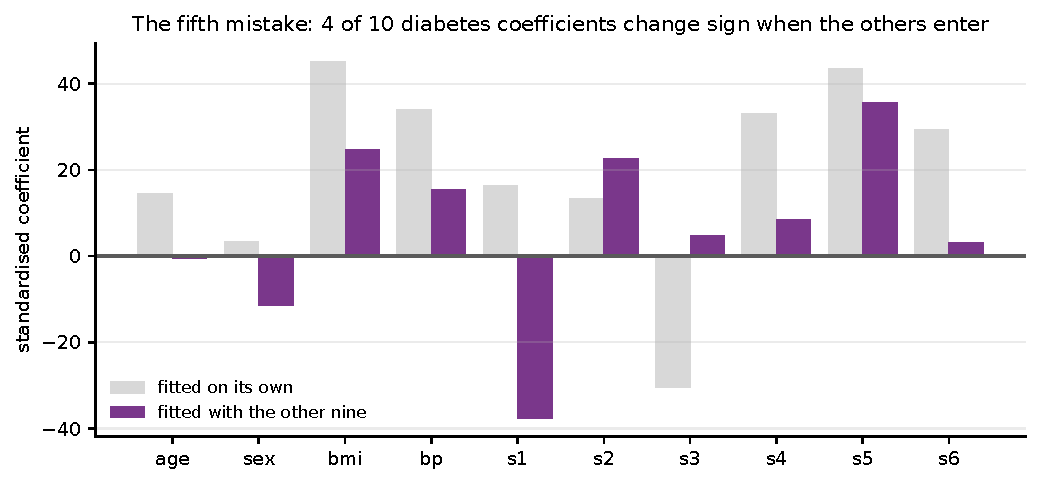
\includegraphics[width=0.72\textwidth,height=0.60\textheight,keepaspectratio]{coefsign.pdf}
  \end{center}
  \vspace{-0.5em}
  \begin{center}
    \small Total serum cholesterol has slope $\mathbf{+0.4723}$ on its own
    and $\mathbf{-1.0900}$ with the other nine predictors present. Both are
    correct. They answer \emph{different questions}.
  \end{center}
\end{frame}

\begin{frame}[shrink=6]{The confounder, built on purpose so the truth is known}
  \begin{columns}[T]
    \begin{column}{0.46\textwidth}
      \begin{block}{The design}
        $Z \sim \mathcal{N}(0,1)$; $X = Z + \varepsilon_1$;
        $Y = 3Z + \varepsilon_2$.\\[0.3em]
        $X$ appears \textbf{nowhere} in the equation for $Y$. Its causal
        effect on $Y$ is exactly zero, by construction.
      \end{block}
    \end{column}
    \begin{column}{0.52\textwidth}
      \begin{exampleblock}{What the regressions say}
        $Y$ on $X$ alone: slope $\mathbf{+2.3662}$, $R^2 = 0.7790$.\\
        $Y$ on $X$ given $Z$: slope $\mathbf{-0.0119}$.\\
        True causal effect: $\mathbf{+0.0000}$.
      \end{exampleblock}
    \end{column}
  \end{columns}
  \vspace{0.3em}
  \begin{alertblock}{The wording that is defensible}
    ``Holding the other predictors in this model fixed, a one-unit increase
    in $x_j$ is \emph{associated with} a change of $b_j$ in the fitted mean
    of $y$.'' Not ``causes''. Not ``if we increase $x_j$''. And never
    without naming which other predictors were in the model.
  \end{alertblock}
\end{frame}

\begin{frame}[fragile,shrink=6]{Predict first \#4 --- find the errors}
\begin{lstlisting}
X = StandardScaler().fit_transform(X)
X = SelectKBest(f_classif, k=20).fit_transform(X, y)
Xtr, Xte, ytr, yte = train_test_split(X, y, test_size=0.2)
gs = GridSearchCV(SVC(), {"C": [0.1, 1, 10]}, cv=5).fit(Xtr, ytr)
print("test accuracy", gs.score(Xte, yte), "best CV", gs.best_score_)
\end{lstlisting}
  \onslide<2->{
  \begin{exampleblock}{Reveal --- there are four}
    \textbf{(1)} the scaler is fitted on all rows, before the split;
    \textbf{(2)} the selector is fitted on all rows \emph{and all labels} ---
    the $+0.2900$ mistake;
    \textbf{(3)} \texttt{train\_test\_split} is not stratified and has no
    \texttt{random\_state};
    \textbf{(4)} \texttt{best\_score\_} is printed beside the test score as
    though the two were comparable estimates. Also: one accuracy on 20\% of
    the rows, with no spread.
  \end{exampleblock}}
\end{frame}

% =====================================================================
\section[End to end]{From raw arrays to a defended result}
\label{sec:e2e}

\begin{frame}{Every step of the course, in the order you would really do it}
  \begin{center}
    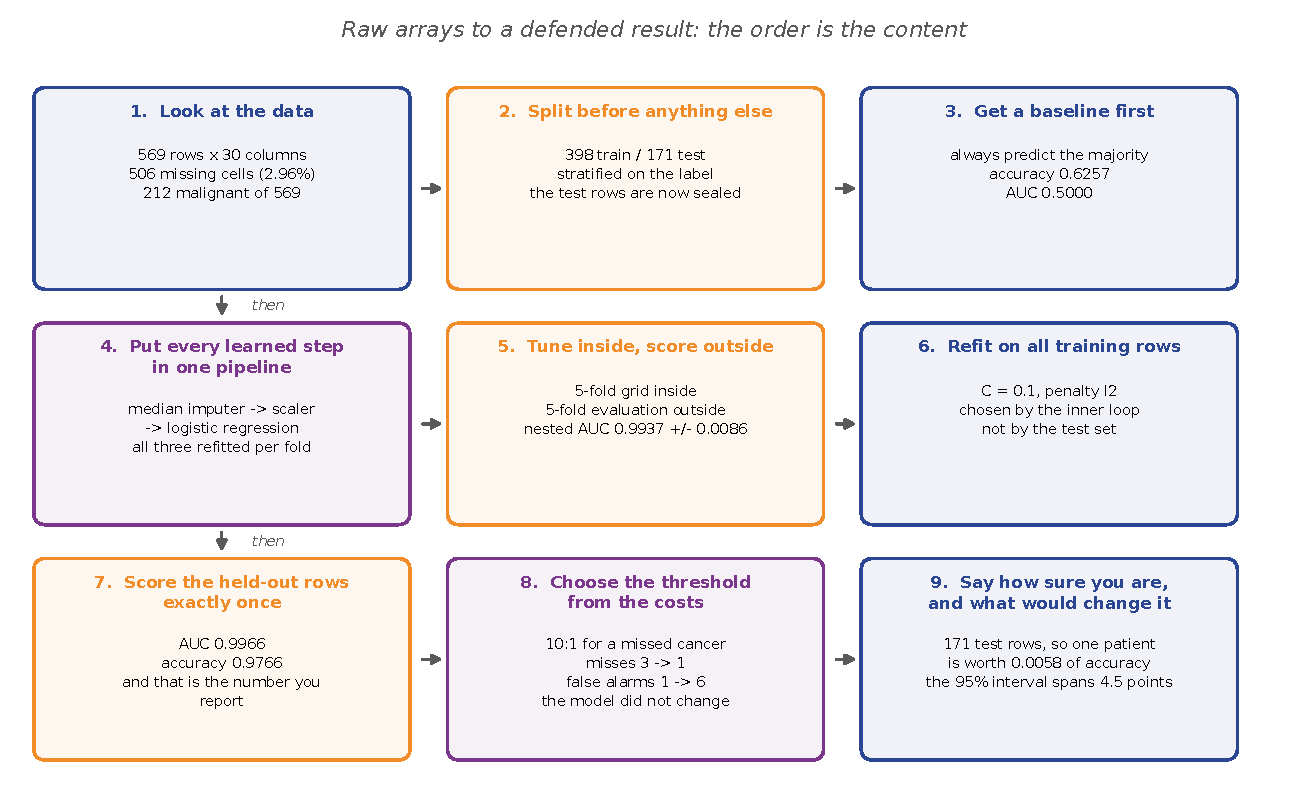
\includegraphics[width=0.86\textwidth,height=0.80\textheight,keepaspectratio]{pipeline.pdf}
  \end{center}
\end{frame}

\begin{frame}[fragile,shrink=4]{Steps 1--3: split, baseline, one pipeline}
\begin{lstlisting}
Xtr, Xte, ytr, yte = train_test_split(X, y, test_size=0.30,
                                      stratify=y, random_state=24)
base = DummyClassifier(strategy="most_frequent").fit(Xtr, ytr)

pipe = Pipeline([("imp", SimpleImputer(strategy="median")),
                 ("sc",  StandardScaler()),
                 ("m",   LogisticRegression(max_iter=5000,
                                            solver="liblinear"))])
\end{lstlisting}
\begin{outblk}
step 0  569 x 30, 506 missing cells (2.96%), 229 complete rows of 569
        positive class = malignant, 212 of 569 rows (0.3726)
step 1  train 398, test 171, prevalence 0.3719 train / 0.3743 test
step 2  majority class: accuracy 0.6257, AUC 0.5000
\end{outblk}
  \begin{center}
    \small Listwise deletion would have thrown away \textbf{340 of 569}
    patients to remove 2.96\% of the cells. That is the exponential
    $(1-p)^d$ from Unit IV, in one line.
  \end{center}
\end{frame}

\begin{frame}[fragile,shrink=4]{Steps 4--6: tune inside, score outside, score once}
\begin{lstlisting}
grid  = {"m__C": [0.001, 0.01, 0.1, 1, 10, 100], "m__penalty": ["l1", "l2"]}
nested = cross_val_score(GridSearchCV(pipe, grid, cv=inner,
                                      scoring="roc_auc"),
                         Xtr, ytr, cv=outer, scoring="roc_auc")
gs = GridSearchCV(pipe, grid, cv=inner, scoring="roc_auc").fit(Xtr, ytr)
\end{lstlisting}
\begin{outblk}
step 4  nested CV on the training rows: AUC 0.9937 +/- 0.0086
step 5  best params {'m__C': 0.1, 'm__penalty': 'l2'}, best_score_ 0.9941
        best_score_ - nested = +0.0004
step 6  held-out rows, scored ONCE: AUC 0.9966, accuracy 0.9766
        confusion matrix  TN 106  FP 1  FN 3  TP 61
        recall 0.9531   precision 0.9839
\end{outblk}
  \begin{center}
    \small The test set was touched exactly once, at step 6, and never again.
    If you look at it and then change something, it is a validation set and
    you no longer have a test set.
  \end{center}
\end{frame}

\begin{frame}[fragile,shrink=5]{Steps 7--8: the threshold is a separate decision}
\begin{outblk}
threshold           TN      FP      FN    recall  precision
0.5000 default     106       1       3    0.9531     0.9839
0.4778 Youden      106       1       3    0.9531     0.9839
0.2525 cost        101       6       1    0.9844     0.9130

step 8  171 test rows: one patient is worth 0.0058 of accuracy;
        binomial se 0.0116, 95% interval [0.9540, 0.9993]
\end{outblk}
  \begin{columns}[T]
    \begin{column}{0.55\textwidth}
      \begin{alertblock}{The number that matters clinically}
        Moving the threshold from $0.5$ to $0.2525$ takes missed
        malignancies from \textbf{3 to 1} and false alarms from 1 to 6.
        \emph{Nothing about the model changed} --- only the price list.
      \end{alertblock}
    \end{column}
    \begin{column}{0.43\textwidth}
      \begin{block}{Reported honestly}
        Youden's $J$, chosen on the out-of-fold scores, picked $0.4778$ and
        \textbf{changed nothing at all} on the test rows. That is what
        happened; it is not a failure of the method, it is what an
        equal-cost rule does on a well-separated problem.
      \end{block}
    \end{column}
  \end{columns}
\end{frame}

\begin{frame}[shrink=6]{Step 9 and 10 --- what a defended result actually says}
  \begin{block}{The sentence to write in a report}
    ``A median-imputed, standardised, $L_2$-penalised logistic regression
    ($C = 0.1$, chosen by a 5-fold inner loop) scored a nested
    cross-validated AUC of \textbf{0.9937 $\pm$ 0.0086} on 398 training
    patients and \textbf{0.9966} on 171 held-out patients, against a
    majority-class baseline of accuracy 0.6257 and AUC 0.5000. At a threshold
    chosen for a 10:1 miss-to-false-alarm cost it missed \textbf{1 of 64}
    malignancies at the price of 6 false alarms. The test set has 171 rows,
    so one patient is worth 0.0058 of accuracy.''
  \end{block}
  \begin{alertblock}{And then the honest caveat}
    ``This is one cohort from one institution. A prevalence shift, a
    different imaging protocol, or a column that encodes the outcome would
    all invalidate it, and none of those is tested here.''
  \end{alertblock}
\end{frame}

% =====================================================================
\section[The arithmetic]{The arithmetic that recurs across units}
\label{sec:hand}

\begin{frame}[shrink=8]{Least squares, and the ridge that generalises it}
  \begin{columns}[T]
    \begin{column}{0.49\textwidth}
      \begin{block}{Five points, all integers}
        $x = (1,2,3,4,5)$, $y = (2,4,5,4,5)$.\\
        $\bar x = 3$, $\bar y = 4$, $S_{xx} = 10$, $S_{xy} = 6$.
        \[
          b_1 = \frac{S_{xy}}{S_{xx}} = 0.6, \qquad
          b_0 = \bar y - b_1 \bar x = 2.2
        \]
        $\mathrm{SSE} = 2.40$, $S_{yy} = 6.00$, $R^2 = 0.6000$,
        $\sum e_i = 0$ and $\sum x_i e_i = 0$.
      \end{block}
    \end{column}
    \begin{column}{0.49\textwidth}
      \begin{block}{Ridge, no intercept, $x=(1,2,2)$, $y=(2,3,5)$}
        \[
          \hat\beta(\lambda) = \frac{x^{\top}y}{x^{\top}x + \lambda}
          = \frac{18}{9 + \lambda}
        \]
        \centering
        \begin{tabular}{@{}lcccc@{}}
          \toprule
          $\lambda$ & 0 & 1 & 9 & 81 \\
          $\hat\beta$ & 2.0 & 1.8 & 1.0 & 0.2 \\
          \bottomrule
        \end{tabular}
      \end{block}
      \begin{center}
        \small \texttt{Ridge} reproduces all four to four decimals.
        $\lambda \to \infty$ shrinks towards zero but never reaches it.
      \end{center}
    \end{column}
  \end{columns}
\end{frame}

\begin{frame}[fragile,shrink=5]{Entropy and information gain --- fourteen rows}
\begin{outblk}
H(S) = H(9/14, 5/14) = 0.940286 bits
Sunny     (2 yes, 3 no)  weight 5/14  H = 0.970951
Overcast  (4 yes, 0 no)  weight 4/14  H = 0.000000
Rain      (3 yes, 2 no)  weight 5/14  H = 0.970951
Remainder(Outlook) = 0.693536   Gain(Outlook) = 0.246750
Gain(Humidity) = 0.151836       Gini(S) = 0.459184
\end{outblk}
  \begin{center}
    \small Outlook wins because it is the only attribute with a \textbf{pure
    child}: four Overcast days, all Yes, entropy exactly 0. That single
    zero-entropy branch is worth $4/14 \times 0.940286 = 0.2686$ of the
    remainder on its own.
  \end{center}
  \begin{alertblock}{The one to remember}
    $H(p) = -\sum p_i \log_2 p_i$; gain $=$ parent entropy minus the
    \emph{weighted} average of the children's. The weights are what stop a
    fourteen-way identifier split from being free.
  \end{alertblock}
\end{frame}

\begin{frame}[fragile,shrink=5]{One backward pass, nine parameters}
  \begin{columns}[T]
    \begin{column}{0.40\textwidth}
      \small
      $x = (1, 0.5)$, target $t = 1$, sigmoid everywhere,
      $L = \tfrac12 (a_2 - t)^2$.\\[0.3em]
      $W^{(1)} = \begin{pmatrix} 0.1 & 0.2 \\ 0.3 & 0.4 \end{pmatrix}$,
      $b^{(1)} = (0.1, 0.1)$,\\[0.3em]
      $W^{(2)} = (0.5, -0.5)$, $b^{(2)} = 0.2$.\\[0.4em]
      $\delta_2 = (a_2 - t)\,a_2(1-a_2)$;\\
      $\delta_1 = \delta_2\, W^{(2)} \odot a_1 \odot (1-a_1)$.
    \end{column}
    \begin{column}{0.58\textwidth}
\begin{outblk}
z1 = [0.300000, 0.600000]  a1 = [0.574443, 0.645656]
z2 = 0.1643931053  a2 = 0.5410059687  L = 0.1053377604
delta2 = -0.1139767142
dL/dW2 = [-0.06547307, -0.07358978]
dL/db2 = -0.11397671
delta1 = [-0.01393128, 0.01303804]
max |analytic - central difference| = 2.095e-11
\end{outblk}
    \end{column}
  \end{columns}
  \begin{center}
    \small One forward pass and one backward pass give \emph{all nine}
    derivatives. Nine separate finite differences would need eighteen forward
    passes --- and that ratio is what makes networks trainable at all.
  \end{center}
\end{frame}

\begin{frame}[shrink=6]{Bayes, and one $k$-means iteration}
  \begin{columns}[T]
    \begin{column}{0.47\textwidth}
      \begin{block}{Prevalence 1\%, sensitivity 99\%, specificity 95\%}
        \[
          P(D \mid +) = \frac{0.99 \times 0.01}{0.99 \times 0.01 +
                              0.05 \times 0.99} = \frac{0.0099}{0.0594}
                      = 0.1667
        \]
        In 10{,}000 people: \textbf{99} true positives arrive alongside
        \textbf{495} false ones. Odds form: $0.010101 \times 19.8 = 0.2$.
      \end{block}
    \end{column}
    \begin{column}{0.50\textwidth}
      \begin{block}{Six points, $k=2$, one Lloyd step}
        Centres $(1,1)$ and $(5,7)$.
        Assignment $\{P_1,P_2,P_3\}$ and $\{P_4,P_5,P_6\}$ --- note $P_3$ is
        \textbf{equidistant} at $3.6056$ and the tie goes to the lower index.
        New centres $(1.8333, 2.3333)$ and $(4.3333, 5.6667)$; $W$ falls from
        $24.7500$ to $\mathbf{10.6667}$.
      \end{block}
    \end{column}
  \end{columns}
  \vspace{0.2em}
  \begin{center}
    \small Both halves of a Lloyd iteration can only decrease $W$, which is
    why $k$-means always terminates --- and why it terminates at a
    \emph{local} minimum.
  \end{center}
\end{frame}

\begin{frame}[fragile,shrink=6]{A confusion matrix, and one point on a ROC curve}
  \begin{columns}[T]
    \begin{column}{0.44\textwidth}
\begin{outblk}
TP 6  FP 2  FN 4  TN 8   (n = 20)
accuracy    0.7000
precision   0.7500
recall      0.6000
specificity 0.8000
FPR         0.2000
F1          0.6667
ROC point   (0.2000, 0.6000)
Youden J    0.4000
\end{outblk}
    \end{column}
    \begin{column}{0.54\textwidth}
      \begin{block}{Ten scored rows $\to$ the whole curve}
        Sort by score, step \emph{up} for a positive and \emph{right} for a
        negative. AUC $= \mathbf{0.8400}$ by trapezoids, and
        $\mathbf{21/25}$ concordant pairs --- the same number, because AUC
        \emph{is} the probability that a random positive outscores a random
        negative.
      \end{block}
      \begin{alertblock}{The trap}
        \texttt{confusion\_matrix} is the \textbf{transpose} of the textbook
        layout: top-left is TN, bottom-right is TP.
      \end{alertblock}
    \end{column}
  \end{columns}
\end{frame}

\begin{frame}[shrink=6]{Predict first \#5 --- three claims, one is defensible}
  \begin{block}{Which of these would you sign your name to?}
    \begin{enumerate}
      \item ``Our model achieves 99.2\% accuracy on fraud detection.''
      \item ``Random forest beat logistic regression, 0.9626 against 0.9767
        --- wait, the other way round --- so we chose the forest.''
      \item ``Nested cross-validated AUC 0.9937 $\pm$ 0.0086; on 171 held-out
        patients, 0.9966; baseline 0.5000.''
    \end{enumerate}
  \end{block}
  \onslide<2->{
  \begin{exampleblock}{Reveal}
    Only \textbf{3}. Claim \textbf{1} quotes accuracy on an imbalanced
    problem --- at 1\% positives, always-say-no scores 0.9900 --- with no
    baseline, no recall and no spread. Claim \textbf{2} picks a winner from a
    gap of $0.0141$ without ever measuring the fold-to-fold spread, which
    here is $0.0163$: \emph{larger than the gap}. Claim \textbf{3} names the
    protocol, the spread, the held-out number and the baseline.
  \end{exampleblock}}
\end{frame}

% =====================================================================
\section[Revision map]{The revision map}
\label{sec:map}

\begin{frame}[shrink=14]{Unit by unit: the one idea, and what is examinable}
  \centering
  \begin{tabular}{@{}p{1.5cm}p{5.6cm}p{6.8cm}@{}}
    \toprule
    \textbf{Unit} & \textbf{The one idea} & \textbf{The calculations that are
      genuinely examinable} \\
    \midrule
    I & Learning is fitting a function from examples; three kinds of task &
      naming the task type; MAE / MSE / RMSE on a handful of numbers \\
    II & Choosing a loss chooses what the model becomes &
      minimising a loss over a constant; MSE $\to$ mean, MAE $\to$ median;
      writing down cross-entropy \\
    III & Step downhill: how big, from how much data, with how much memory &
      one gradient-descent step by hand; the divergence condition; one
      momentum and one Adam update \\
    IV & What you feed it decides what it can find &
      $(1-p)^d$ row survival; the $z$, IQR and modified-$z$ rules; a
      standardisation by hand; what belongs inside the fold \\
    V & Least squares has an answer you can write down, and $\lambda$
      controls it &
      $b_1 = S_{xy}/S_{xx}$; $R^2$; the normal equations on a $2 \times 2$;
      ridge $\hat\beta = X^\top y / (X^\top X + \lambda)$; soft thresholding \\
    VI & One recipe, several hypothesis classes &
      entropy and information gain; a 1-NN by hand; Bayes with a prior; one
      AdaBoost round; one forward and backward pass; the margin on
      six points \\
    VII & Remove the target and the distance becomes the whole decision &
      a proximity matrix; single against complete linkage to completion; one
      Lloyd iteration; silhouette for one point \\
    \bottomrule
  \end{tabular}
\end{frame}

\begin{frame}[shrink=8]{What to reread, and in what order}
  \begin{columns}[T]
    \begin{column}{0.49\textwidth}
      \begin{block}{If you have one evening}
        The four boxes of the spine figure, and then the six by-hand
        calculations in Section~\ref{sec:hand}: least squares, information
        gain, one backward pass, Bayes, one Lloyd iteration, and a confusion
        matrix with its ROC point. Those six recur across the whole paper.
      \end{block}
    \end{column}
    \begin{column}{0.49\textwidth}
      \begin{block}{If you have a week}
        Add the derivations: why least squares is the Gaussian MLE, why
        $X^\top X + \lambda I$ is always invertible, why the logistic
        log-likelihood is concave, why a bootstrap sample holds $63.2\%$ of
        the unique rows, and why single linkage chains.
      \end{block}
    \end{column}
  \end{columns}
  \begin{alertblock}{What is \emph{not} worth memorising}
    Library argument names. The exact coefficient table of Lance--Williams.
    Any number you can recompute in ten seconds. Spend the time on the
    arithmetic you can be asked to \emph{produce} rather than recognise.
  \end{alertblock}
\end{frame}

% =====================================================================
\section[Assessment]{What is left to be assessed}
\label{sec:assess}

\begin{frame}[shrink=8]{The remaining internal components}
  \begin{block}{What is still to come}
    \begin{itemize}
      \item \textbf{Theory quizzes.} T10 is the last of the ten, covering
        Unit VII's algorithms --- hierarchical, partitioning and
        density-based clustering. 40 minutes, like every other one.
      \item \textbf{Lab assignments and lab quizzes.} LA10 covers experiments
        13 and 14; LQ10 follows it. Each lab quiz is 60 minutes at the
        machine, on \emph{your own} submitted code.
      \item \textbf{Project.} Final submission --- code, report and
        reproducibility notes --- and then the \textbf{individual project
        quiz}.
    \end{itemize}
  \end{block}
  \begin{alertblock}{Dates}
    Every remaining date is announced on the LMS and in class, at least one
    session ahead. Do not infer one from the syllabus.
  \end{alertblock}
\end{frame}

\begin{frame}[shrink=8]{The project quiz, since it is the largest single piece left}
  \begin{columns}[T]
    \begin{column}{0.49\textwidth}
      \begin{block}{How it is structured}
        Of the 15 project marks, \textbf{10 are individual} --- an oral and
        written test on your own group's project, with everyone asked
        separately --- and \textbf{5 are for the group}, awarded for the
        state of what was submitted: completeness, correctness,
        reproducibility, documentation.
      \end{block}
    \end{column}
    \begin{column}{0.49\textwidth}
      \begin{block}{What it asks for}
        Your project, in your words: what problem, what data, what you
        cleaned and why, what models you compared, on what protocol, with
        what spread, and what you would do differently. Every one of those is
        a question this course has an answer to.
      \end{block}
    \end{column}
  \end{columns}
  \begin{alertblock}{The one preparation that helps}
    Be able to run your own pipeline end to end and explain each line of it.
    Two thirds of the project mark is individual, so a strong contributor in
    a weak group can still score well --- and the reverse is also true.
  \end{alertblock}
\end{frame}

\begin{frame}[shrink=6]{What good work looks like from here}
  \begin{columns}[T]
    \begin{column}{0.49\textwidth}
      \begin{block}{In the report}
        A baseline. A pipeline with every learned step inside it. A
        cross-validated score \emph{with its spread}. One held-out number,
        scored once. A metric chosen from the problem. A threshold chosen
        from the costs. And a paragraph on what would change your mind.
      \end{block}
    \end{column}
    \begin{column}{0.49\textwidth}
      \begin{block}{In the viva}
        Why that model and not another --- naming a property of the data.
        Why that metric. What the spread was. What you tried that did not
        work, reported as it happened. A null result you can explain is
        worth more than a good number you cannot.
      \end{block}
    \end{column}
  \end{columns}
  \begin{center}
    \small Reproducibility is a mark, not a courtesy: a fixed seed, a pinned
    version list, and a script that runs from a clean checkout.
  \end{center}
\end{frame}

% =====================================================================
\section{Summary}
\label{sec:summary}

\begin{frame}[shrink=10]{What to carry out of this course}
  \begin{columns}[T]
    \begin{column}{0.49\textwidth}
      \begin{block}{The argument}
        \begin{enumerate}
          \item Choose a loss --- it decides what the model becomes.
          \item Minimise it --- the how does not depend on the what.
          \item Over a class of functions --- the class is the modelling
            decision, and it is a statement about the shape you believe the
            answer has.
          \item On columns you chose --- and everything you learn from the
            data belongs inside the fold.
          \item Prove it on data the fit never saw --- with the spread.
        \end{enumerate}
      \end{block}
    \end{column}
    \begin{column}{0.49\textwidth}
      \begin{alertblock}{The five numbers}
        $+0.2900$ --- a selector outside the pipeline.\\
        $+0.0515$ --- tuning and scoring on the same folds.\\
        $0.9900$ --- the accuracy of doing nothing at 1\% positives.\\
        $+0.0633$ --- an RBF SVM with a scaler in front of it.\\
        $+0.4723 \to -1.0900$ --- a coefficient that is not a cause.
      \end{alertblock}
      \begin{exampleblock}{And the honest one}
        On this dataset, seven very different models are separated by less
        than the fold-to-fold noise. \textbf{The method is rarely the thing
        that decides the answer.} The data, the columns and the protocol are.
      \end{exampleblock}
    \end{column}
  \end{columns}
\end{frame}

\begin{frame}{Where to go next}
  \begin{columns}[T]
    \begin{column}{0.49\textwidth}
      \begin{block}{Immediately}
        The notes for this lecture carry a \textbf{revision map} for all
        seven units, fifteen practice questions weighted towards the
        recurring hand calculations, and full worked solutions.
      \end{block}
    \end{column}
    \begin{column}{0.49\textwidth}
      \begin{block}{Afterwards}
        Convolutional and recurrent networks, probabilistic graphical models,
        reinforcement learning, and the whole of deployment --- monitoring,
        drift, fairness. Everything in this course is the vocabulary those
        subjects assume.
      \end{block}
    \end{column}
  \end{columns}
  \vspace{0.6em}
  \begin{center}
    \large It has been a pleasure. Go and measure something.
  \end{center}
  \slidesources{\AMLPrescribed}
\end{frame}

\end{document}
